\documentclass[10pt,aspectratio=169]{beamer}

\usetheme[numbering=fraction,progressbar=foot]{metropolis}

\usepackage[T1]{fontenc}
\usepackage{lmodern}
\usepackage{microtype}
\usepackage{booktabs}
\usepackage{array}
\usepackage{graphicx}
\usepackage{tikz}
\usepackage{openmoji}

\usetikzlibrary{arrows.meta,calc,positioning,shapes.geometric}

\definecolor{Ink}{HTML}{1F2937}
\definecolor{Muted}{HTML}{6B7280}
\definecolor{Sand}{HTML}{F7F4EC}
\definecolor{Gold}{HTML}{C27D38}
\definecolor{Teal}{HTML}{147A73}
\definecolor{Sage}{HTML}{6B8F71}
\definecolor{Rose}{HTML}{C85C5C}
\definecolor{Paper}{HTML}{FFFDF8}
\definecolor{Mist}{HTML}{E8F1EF}
\definecolor{Peach}{HTML}{F6E4D8}
\definecolor{Slate}{HTML}{DDE4EC}

\setbeamercolor{normal text}{fg=Ink,bg=Sand}
\setbeamercolor{frametitle}{fg=Ink,bg=Sand}
\setbeamercolor{progress bar}{fg=Gold,bg=Slate}
\setbeamercolor{title separator}{fg=Gold}
\setbeamercolor{alerted text}{fg=Gold}
\setbeamercolor{footnote}{fg=Muted}

\setbeamertemplate{navigation symbols}{}
\setbeamertemplate{footline}[frame number]
\setbeamersize{text margin left=0.75cm,text margin right=0.75cm}

\title{Deep Generative Genre Remastering}
\subtitle{From ``coat-of-paint'' transfer to structure-aware genre reconstruction}
\author{Sahara Kaul \and Kelsey Pattison \and Ahmed Sajid}
\date{CMPUT 414, Winter 2026}

\newcommand{\cardbox}[2]{%
  \begin{tikzpicture}
    \node[
      fill=#1,
      rounded corners=14pt,
      inner xsep=12pt,
      inner ysep=10pt,
      text width=\dimexpr\linewidth-24pt\relax,
      align=left
    ] {\strut #2};
  \end{tikzpicture}%
}

\newcommand{\tagpill}[2]{%
  \tikz[baseline=(x.base)]\node[
    fill=#1,
    rounded corners=7pt,
    inner xsep=7pt,
    inner ysep=3.5pt
  ] (x) {\scriptsize\bfseries #2};%
}

\newcommand{\labnode}[5]{%
  \node[
    rounded corners=16pt,
    fill=#1,
    inner xsep=10pt,
    inner ysep=10pt,
    text width=0.205\linewidth,
    minimum height=2.35cm,
    align=left
  ] (#2) at #3 {#4\\[0.35em]{\scriptsize #5}};
}

\begin{document}

\begin{frame}[plain]
\begin{tikzpicture}[remember picture,overlay]
  \fill[Teal!20] ($(current page.south west)+(-0.6,0.4)$) circle (2.8cm);
  \fill[Gold!25] ($(current page.north east)+(-0.8,-0.8)$) circle (2.5cm);
  \fill[Rose!12] ($(current page.north west)+(1.4,-0.7)$) circle (1.4cm);
\end{tikzpicture}

\vspace{0.5cm}
\begin{columns}[T,onlytextwidth]
  \column{0.6\textwidth}
  {\usebeamerfont{title}\color{Ink}\inserttitle\par}
  \vspace{0.3cm}
  {\large\color{Muted}\insertsubtitle\par}
  \vspace{0.65cm}
  {\normalsize\insertauthor\par}
  {\small\color{Muted}\insertdate\par}
  \vspace{0.6cm}
  {\small
  \tagpill{Mist}{Problem}
  \hspace{0.4em}
  surface timbre transfer sounds filtered, not re-composed.}
  \par\vspace{0.3cm}
  {\small
  \tagpill{Peach}{Thesis}
  \hspace{0.4em}
  deconstruct content vs style, then rebuild audio inside a target genre space.}

  \column{0.4\textwidth}
  \cardbox{Paper}{
    \textbf{\openmoji[height=1.5ex]{musical score} Core pipeline}\\[-0.1em]
    \small
    Lab 1: disentangle content and style\\
    Lab 2: calibrate a 160D target vector\\
    Lab 3: remaster with codec and diffusion branches\\
    Lab 4: extend to coherent long-form audio
  }
  \vspace{0.25cm}
  \cardbox{Mist}{
    \textbf{\openmoji[height=1.5ex]{sparkles} Demo claim}\\[-0.1em]
    \small
    Short-form genre remastering already clears our main project gates; long-form coherence is measurable and improving.
  }
\end{columns}
\end{frame}

\begin{frame}{Why This Problem Is Hard}
\begin{columns}[T,onlytextwidth]
  \column{0.5\textwidth}
  \cardbox{Peach}{
    \textbf{\openmoji[height=1.4ex]{speaker high volume} 1. Surface transfer is not enough}\\[-0.15em]
    \scriptsize
    Earlier audio style transfer often changed timbre while leaving arrangement untouched. The result sounds filtered, not genuinely re-authored.
  }
  \vspace{0.22cm}
  \cardbox{Mist}{
    \textbf{\openmoji[height=1.4ex]{brain} 2. Music is entangled at multiple levels}\\[-0.15em]
    \scriptsize
    Melody, rhythm, harmony, articulation, and texture are coupled. Without disentanglement, style edits also damage the melodic skeleton.
  }

  \column{0.5\textwidth}
  \cardbox{Slate}{
    \textbf{\openmoji[height=1.4ex]{control knobs} 3. What the literature points toward}\\[-0.15em]
    \scriptsize
    Dai et al. identify the ``coat-of-paint'' problem; Hung and Yang show disentanglement; Roberts, Ho, and Meng motivate structure-aware generation with source anchoring.
  }
  \vspace{0.22cm}
  \cardbox{Paper}{
    \textbf{\openmoji[height=1.4ex]{sparkles} Our project hypothesis}\\[-0.15em]
    \scriptsize
    Genre remastering should preserve structure, replace the style blueprint, and reconstruct with a generator that respects audio realism instead of just repainting the waveform.
  }
\end{columns}

\vspace{0.12cm}
{\tiny\color{Muted}Literature anchors: Dai et al. (2018), Hung et al. (2019), Yang et al. (2019), Roberts et al. (2018), Ho et al. (2020), Meng et al. (2022).}
\end{frame}

\begin{frame}[shrink=6]{What We Built}
\begin{tikzpicture}[remember picture,overlay]
  \fill[Paper] ($(current page.north west)+(0.35,-1.3)$) rectangle ($(current page.south east)+(-0.35,1.05)$);
\end{tikzpicture}

\vspace{0.1cm}
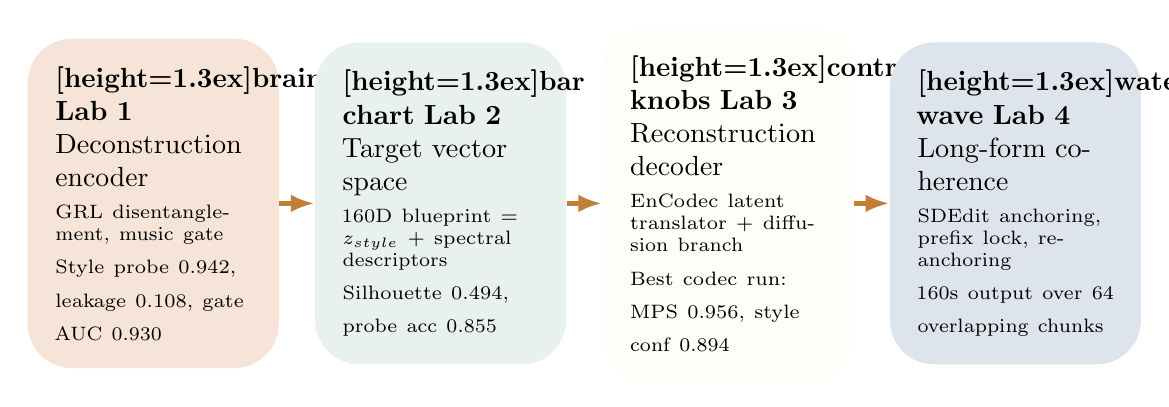
\begin{tikzpicture}[>=Latex]
  \labnode{Peach}{lab1}{(1.35,0)}{\textbf{\openmoji[height=1.3ex]{brain} Lab 1}\\Deconstruction encoder}{GRL disentanglement, music gate\\Style probe 0.942, leakage 0.108, gate AUC 0.930}
  \labnode{Mist}{lab2}{(5.0,0)}{\textbf{\openmoji[height=1.3ex]{bar chart} Lab 2}\\Target vector space}{160D blueprint = $z_{style}$ + spectral descriptors\\Silhouette 0.494, probe acc 0.855}
  \labnode{Paper}{lab3}{(8.65,0)}{\textbf{\openmoji[height=1.3ex]{control knobs} Lab 3}\\Reconstruction decoder}{EnCodec latent translator + diffusion branch\\Best codec run: MPS 0.956, style conf 0.894}
  \labnode{Slate}{lab4}{(12.3,0)}{\textbf{\openmoji[height=1.3ex]{water wave} Lab 4}\\Long-form coherence}{SDEdit anchoring, prefix lock, re-anchoring\\160s output over 64 overlapping chunks}

  \draw[-{Latex[length=3mm]}, ultra thick, color=Gold] (lab1.east) -- (lab2.west);
  \draw[-{Latex[length=3mm]}, ultra thick, color=Gold] (lab2.east) -- (lab3.west);
  \draw[-{Latex[length=3mm]}, ultra thick, color=Gold] (lab3.east) -- (lab4.west);
\end{tikzpicture}

\vspace{0.2cm}
\begin{columns}[T,onlytextwidth]
  \column{0.5\textwidth}
  \cardbox{Mist}{
    \textbf{Engineering decisions that changed the results}\\[-0.15em]
    \scriptsize
    1. EnCodec as a decoder guardrail to avoid raw-audio instability.\\
    2. MERT-probe embeddings for cleaner style conditioning.\\
    3. Direct-output translator to remove the residual style ceiling.
  }

  \column{0.5\textwidth}
  \cardbox{Peach}{
    \textbf{Progress by lab}\\[-0.15em]
    \scriptsize
    Labs 1--4 are implemented in code, notebooks, and saved runs. Lab 5 already has listening-panel tooling, but the final blind study is still pending rather than part of our current evidence.
  }
\end{columns}
\end{frame}

\begin{frame}[shrink=4]{Measured Progress}
\begin{columns}[T,onlytextwidth]
  \column{0.62\textwidth}
  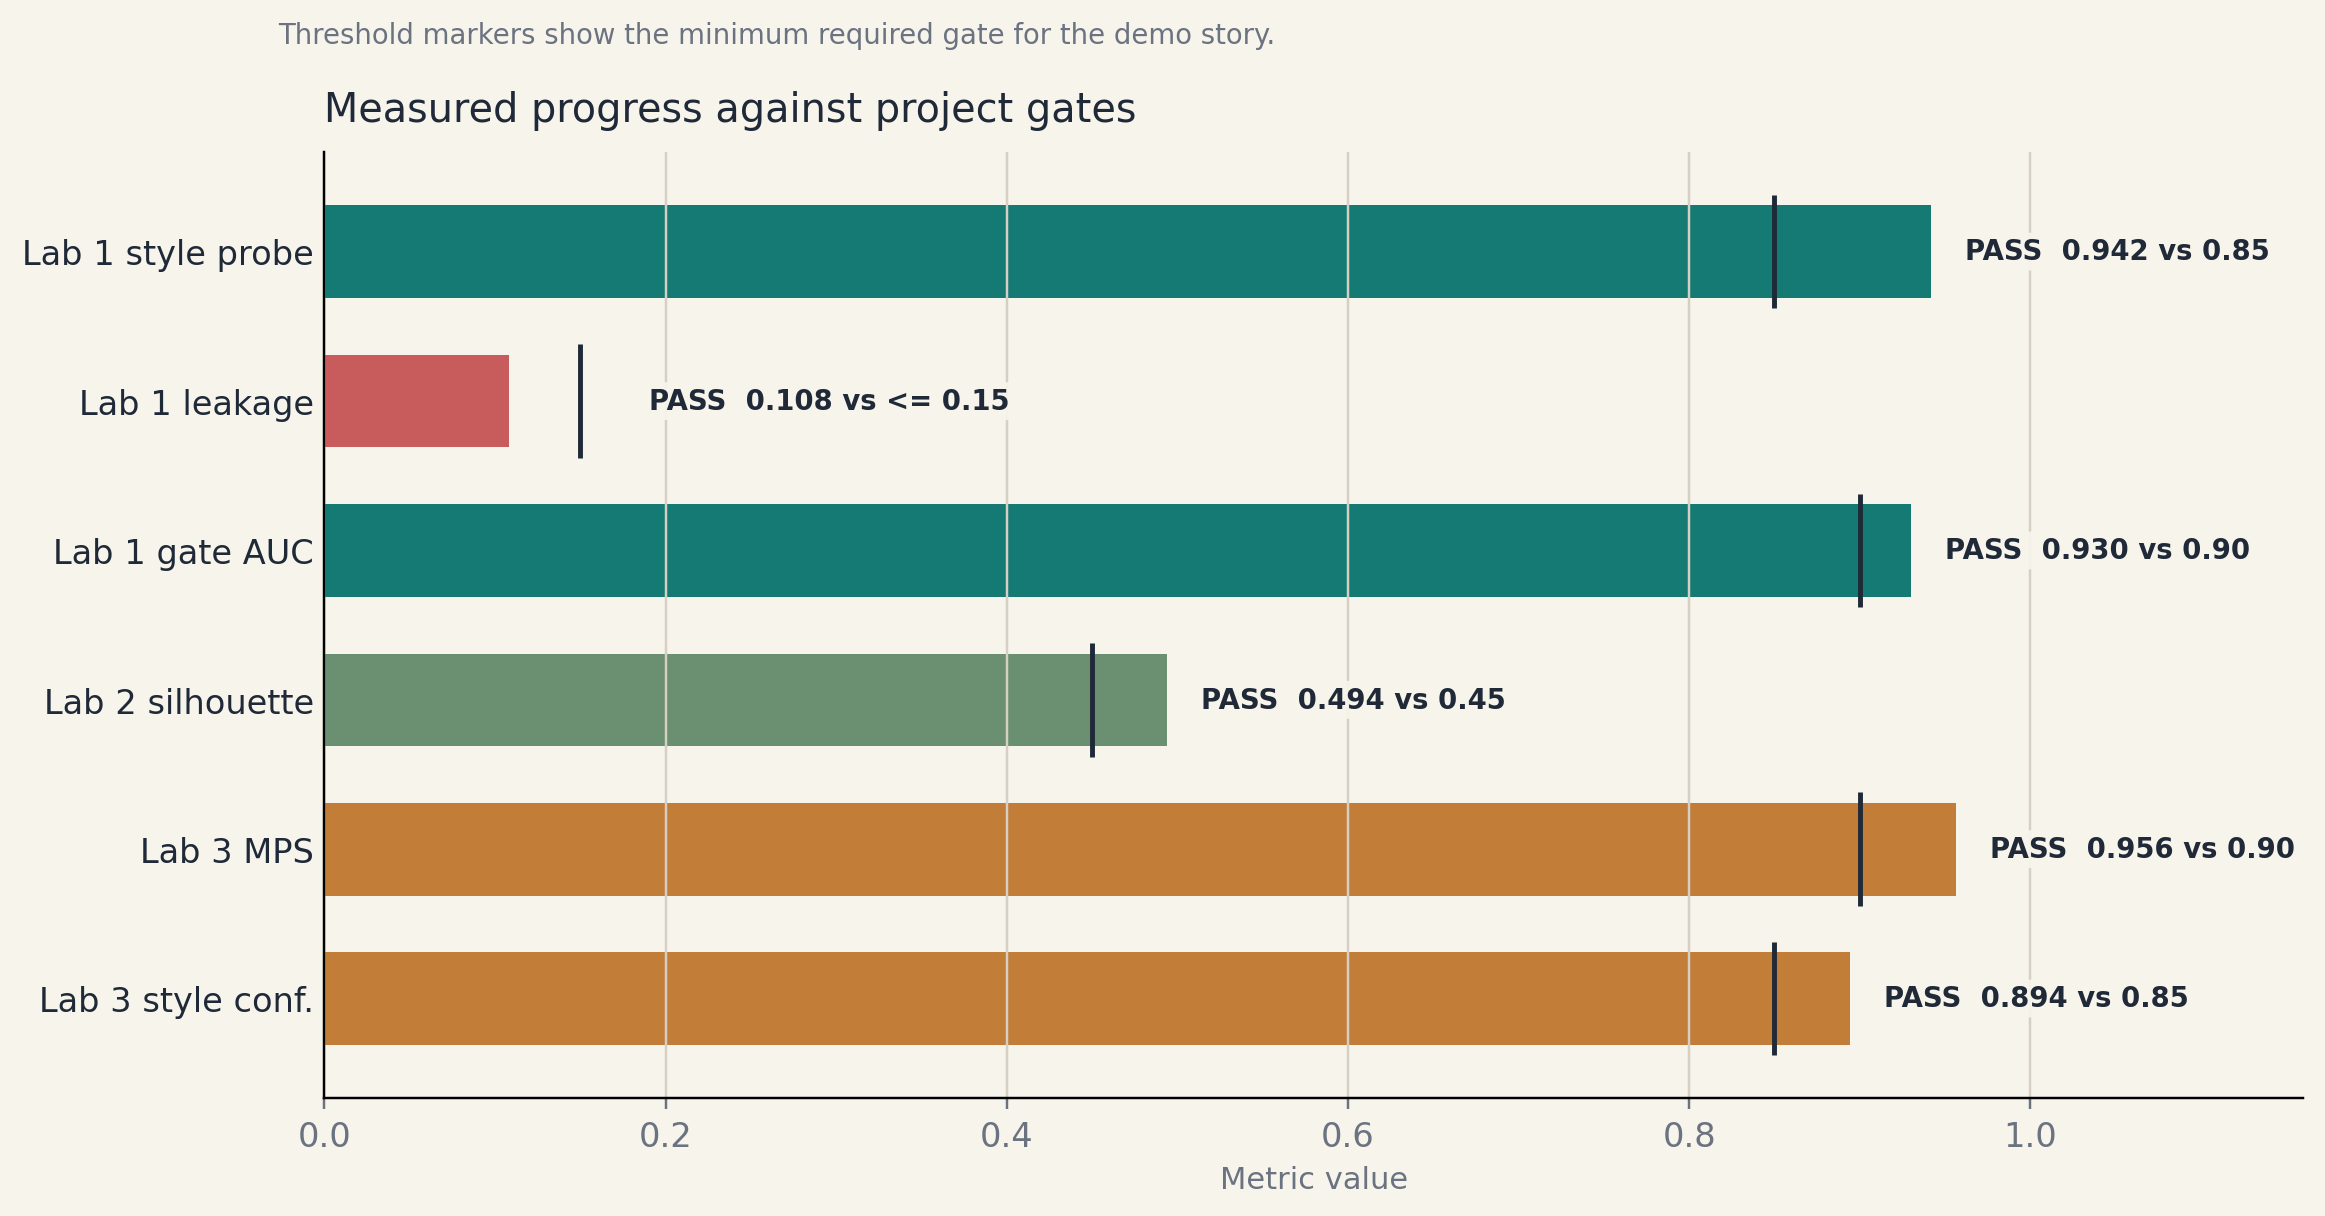
\includegraphics[width=\linewidth,height=0.69\textheight,keepaspectratio]{assets/metrics_dashboard.png}

  \column{0.38\textwidth}
  \cardbox{Paper}{
    \textbf{\openmoji[height=1.4ex]{chart increasing} Main result}\\[-0.15em]
    \scriptsize
    The project gates in Labs 1--3 are now measured wins, not just planned targets.
    \vspace{0.2cm}

    \textbf{Best short-form run}\\[-0.15em]
    \scriptsize
    \texttt{run1055} is the strongest demo candidate:
    MPS $= 0.956$,
    style confidence $= 0.894$,
    style accuracy $= 0.949$.
  }
  \vspace{0.2cm}
  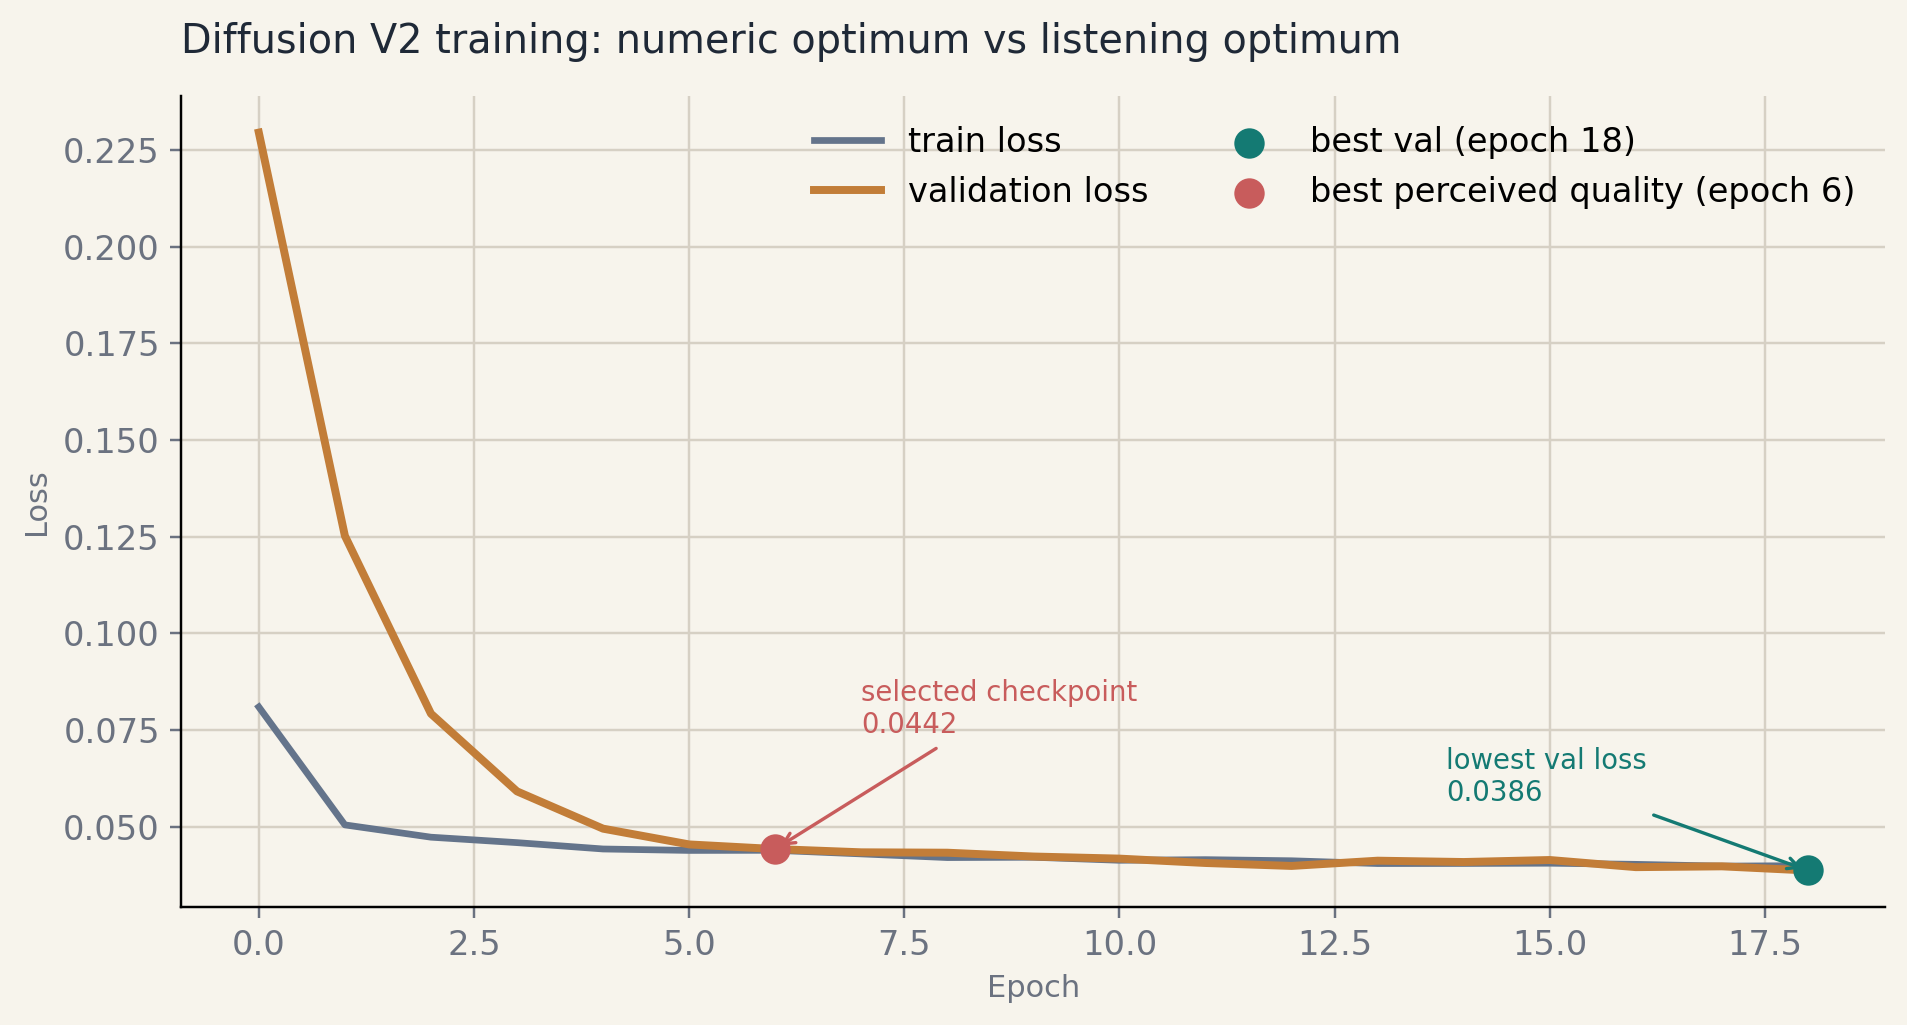
\includegraphics[width=\linewidth,height=0.29\textheight,keepaspectratio]{assets/diffusion_v2_curve.png}
\end{columns}

\vspace{0.12cm}
{\scriptsize\color{Muted}Interpretation: the codec branch is currently our most reliable demo path, while diffusion remains important because it gives stronger edit freedom and enabled the long-form experiments.}
\end{frame}

\begin{frame}[shrink=8]{Long-Form Coherence and Demo Story}
\begin{columns}[T,onlytextwidth]
  \column{0.6\textwidth}
  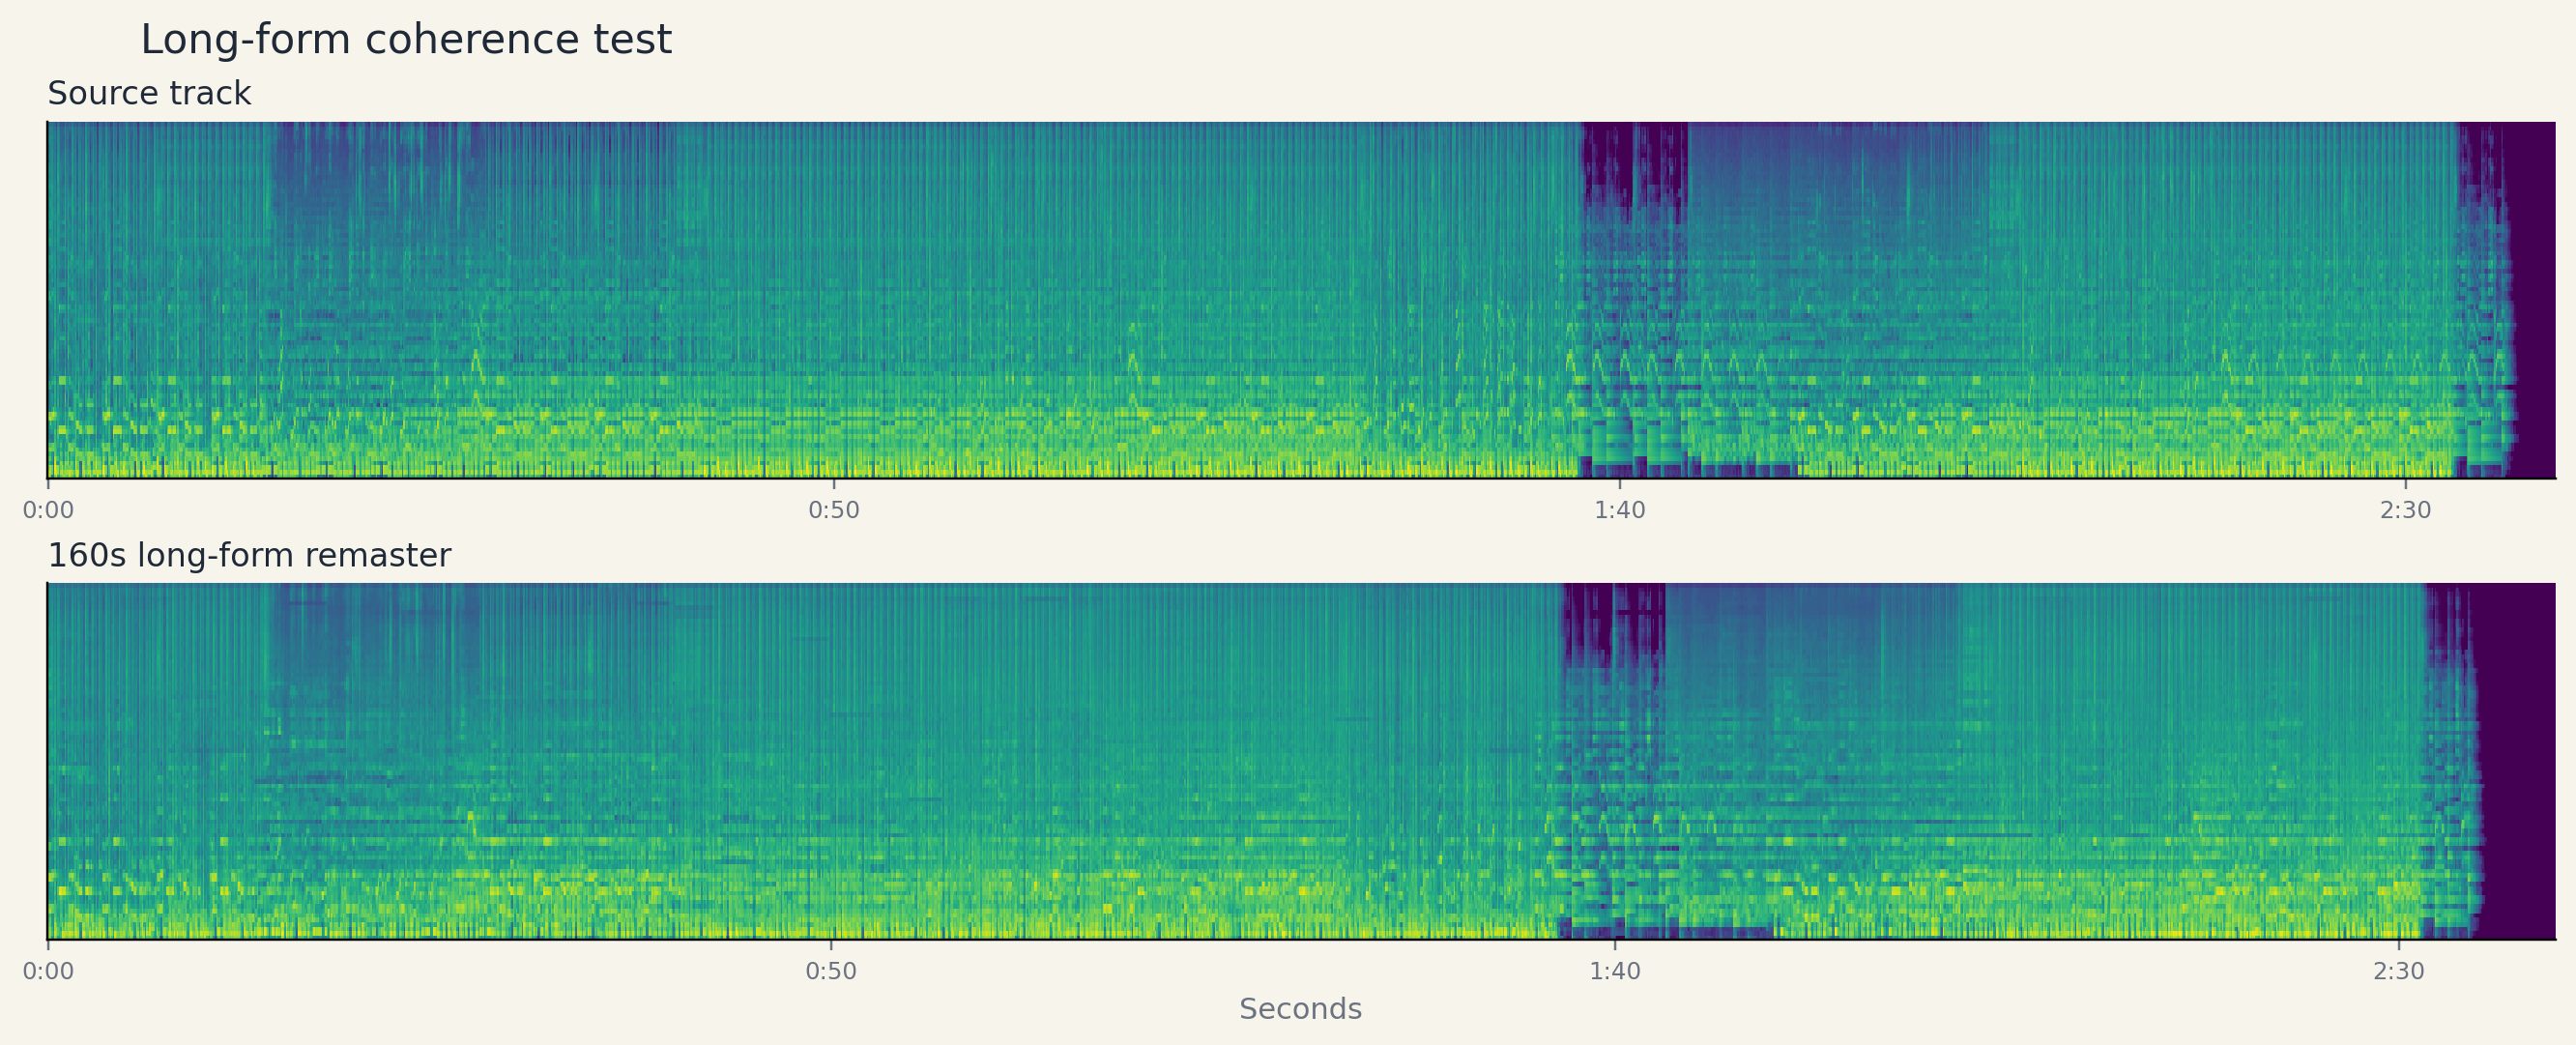
\includegraphics[width=\linewidth,height=0.73\textheight,keepaspectratio]{assets/longform_comparison.png}

  \column{0.4\textwidth}
  \cardbox{Mist}{
    \textbf{\openmoji[height=1.4ex]{musical notes} What Lab 4 shows}\\[-0.15em]
    \scriptsize
    We can remaster a full 160-second track by stitching 64 overlapping chunks while keeping the structure visibly coherent over time.
  }
  \vspace{0.18cm}
  \cardbox{Paper}{
    \textbf{Coherence metrics}\\[-0.15em]
    \scriptsize
    boundary mel MSE mean: \textbf{0.00183}\\
    boundary discontinuity mean: \textbf{2.87 dB}\\
    Remaining issue: perceptual warble/static accumulation, not hard seams.
  }
  \vspace{0.18cm}
  \cardbox{Peach}{
    \textbf{How we will present the demo}\\[-0.15em]
    \scriptsize
    Show the DGGR pipeline, play 2 short codec remasters from \texttt{run1055}, then play 1 long-form sample and close with Lab 5 as the final human-validation layer.
  }
\end{columns}
\end{frame}

\appendix

\begin{frame}[noframenumbering]{Backup: Example Short-Form Outputs}
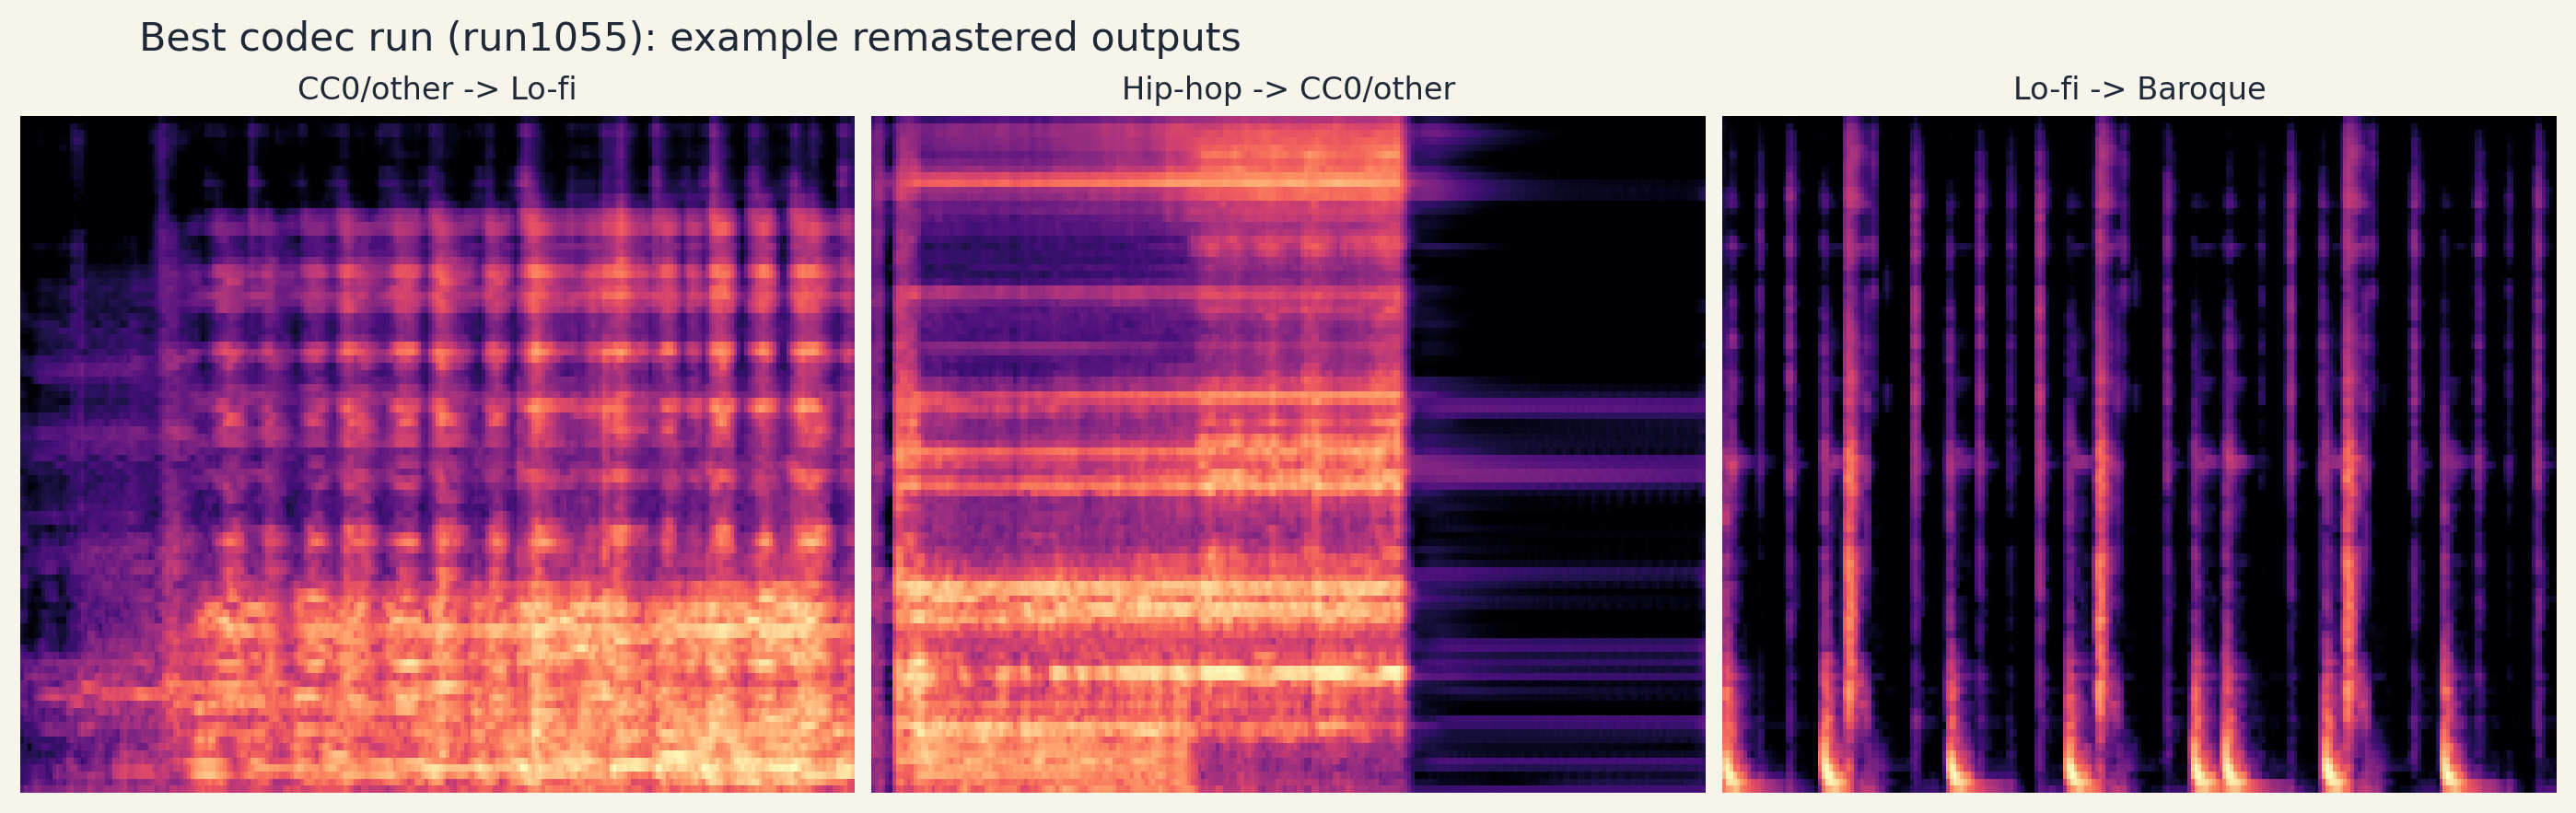
\includegraphics[width=\linewidth]{assets/codec_gallery.png}

\vspace{0.2cm}
{\small\color{Muted}All three clips are drawn from the shipped example set in \texttt{examples/audio/} and come from the best codec transfer run, \texttt{run1055}.}
\end{frame}

\begin{frame}[noframenumbering]{Backup: Sources and Visual Credits}
\small
\textbf{Primary project references}\\
\footnotesize
Dai et al. (2018), Hung et al. (2019), Yang et al. (2019), Roberts et al. (2018), Donahue et al. (2019), Engel et al. (2019), Ho et al. (2020), Ho and Salimans (2021), Meng et al. (2022), Lee et al. (2023), Perez et al. (2018).

\vspace{0.4cm}
\textbf{Repo-backed evidence used in these slides}\\
\footnotesize
Lab 1 audit summaries under \texttt{saves/lab1\_run\_combo\_af\_gate\_exit\_v2/}, Lab 2 validation summary under \texttt{saves/lab2\_calibration/lab2\_20260211\_015118\_lda\_cleanup\_v2/}, Lab 3 codec metrics under \texttt{saves2/lab3\_codec\_transfer/run1055/}, diffusion history under \texttt{saves2/lab3\_diffusion/run\_d002/}, and long-form metrics under \texttt{saves2/lab4\_longform\_coherence/fullsong\_test/}.

\vspace{0.4cm}
\textbf{Visual credits}\\
\footnotesize
OpenMoji icons via the local \texttt{openmoji} LaTeX package (CC BY-SA 4.0). Charts and spectrograms were generated locally from repo artifacts using \texttt{presentation/generate\_figures.py}.
\end{frame}

\end{document}
